\subsection{Heading autopilot}\label{subsec:prob1.1}
\subsubsection*{Analysis of ship characteristics}
To be able to model the ship in a good way we ran many simulations with different rudder angle and measured the steady-state yaw rate. We then made a $\delta-r$ plot of the result. Since the ship was turning port while giving a positive rudder command, this plot and the rest of the assignment is made with a fixed gain of -1 on $\delta_c$.
\begin{figure}[H]
    \centering
    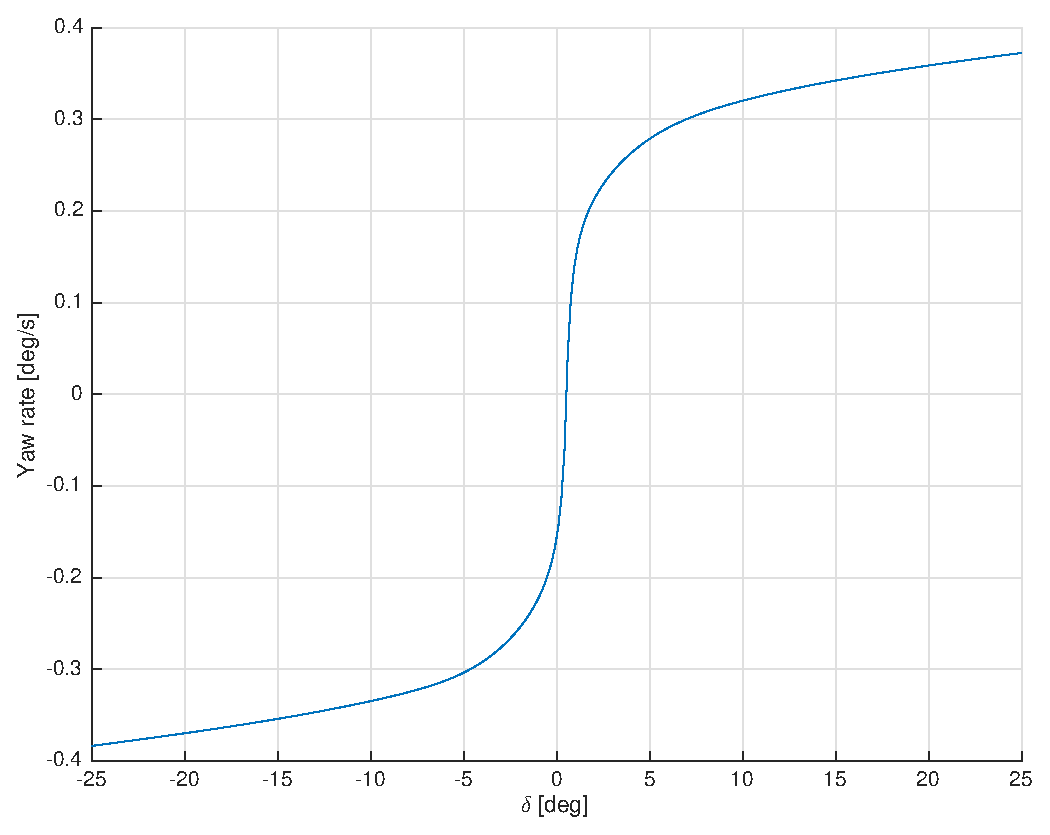
\includegraphics[width=0.9 \textwidth]{task1.4/Task1_4_delta_r_plot}
    \caption{$\delta - r$ plot}
    \label{fig:delta-r-plot}
\end{figure}
From figure \ref{fig:delta-r-plot} we clearly see the non-linear characteristics of the ship. Since we only want to control heading and course, a 1-DOF heading model i.e. first- or second order Nomoto model with or without non-linear extensions can be used. To further investigate the effect of the non-linear characteristics of this ship, we compare the actual response with different models at different rudder angles. It should also be noticed that the ship has a constant drift to starboard when $\delta_c=0$ as seen by the curve not passing through the origin. We compensate for this through the rest of the modeling part by adding a fixed rudder angle of $0.52\degree$ to the rudder input. We only need this correction while estimating the model parameters. In a closed loop, the integral effect will cancel both this drift and drift caused by wind, current and waves.

\subsubsection*{2. order linear Nomoto model}

\begin{equation}
	\frac{r}{\delta}(s) = \frac{K(1+T_3 s)}{(1+T_1 s) (1+T_2 s) } \\
\end{equation}

The second order Nomoto model follows the ship´s overshoot quite well. 

\begin{figure}[H]
    \centering
    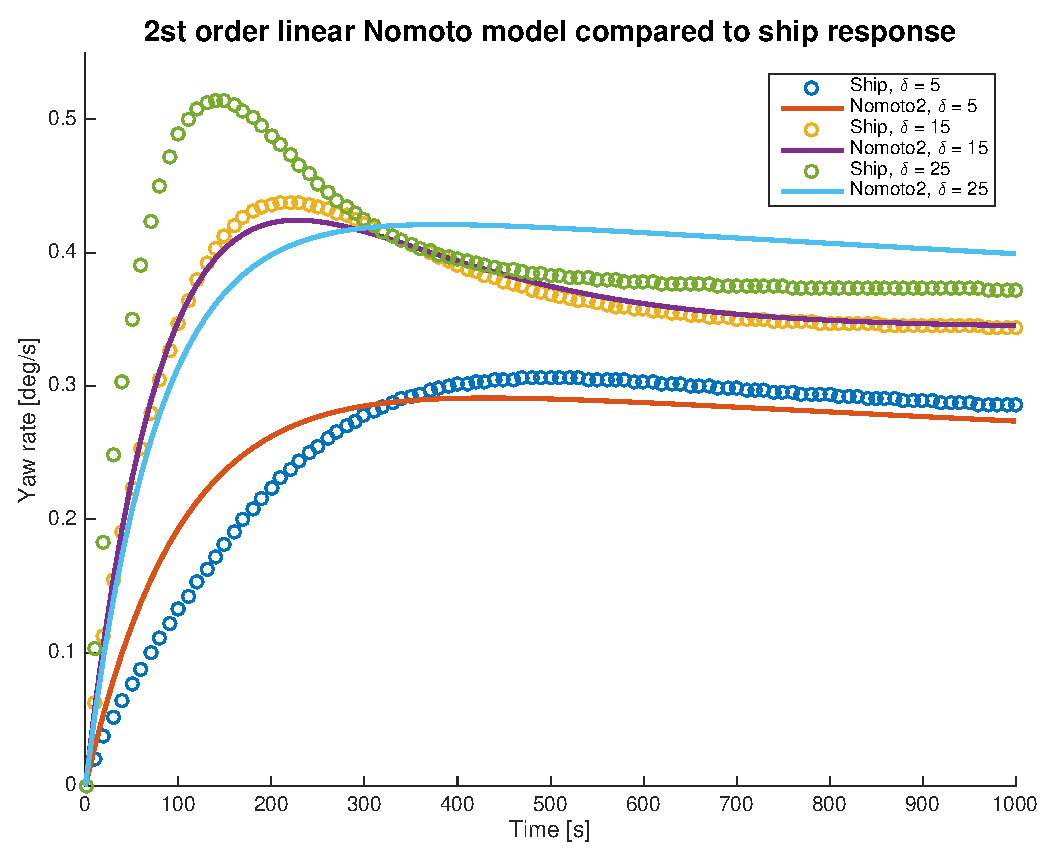
\includegraphics[width= \textwidth]{task1.4/Task1_4_Nomoto2}
    \caption{2.order linear Nomoto model}
    \label{fig:nomoto2_lin}
\end{figure}

\newpage
\subsubsection*{1. order linear Nomoto}

\begin{equation}
	\frac{r}{\delta}(s) = \frac{K}{(1+Ts) } \\
\end{equation}

We also tried the first order version Nomoto, and as expected the model will only be accurate for small rudder angles, and is therefore not very good for modeling the overshoot and non-linearities.

\begin{figure}[H]
    \centering
    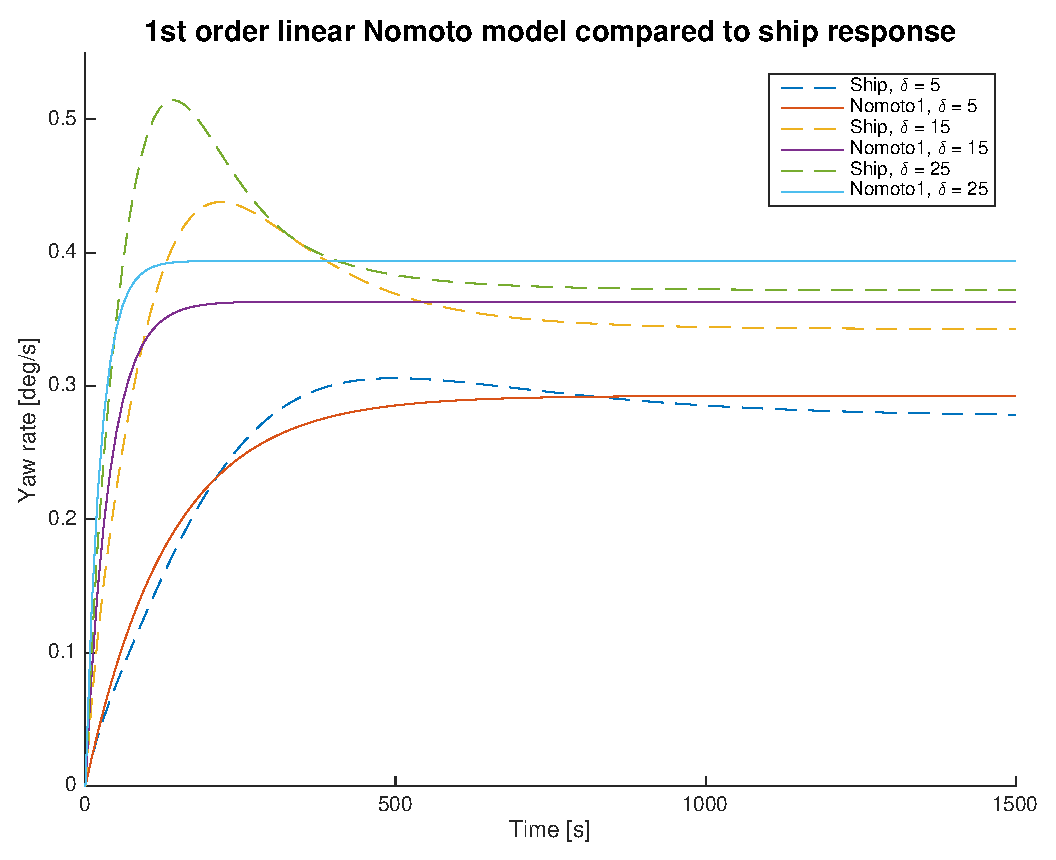
\includegraphics[width= \textwidth]{task1.4/Task1_4_Nomoto1}
    \caption{1.order linear Nomoto model}
    \label{fig:nomoto1_lin}
\end{figure}

\newpage
\subsubsection*{2. order non-linear Nomoto}
\begin{equation}
\begin{split}
	T_1 T_2 \ddot{r} + (T_1 + T_2)\dot{r} + KH_B(r) &= K(\delta + T_3\dot{\delta}) \\
	H_B(r) &= b_3r^3 + b_2r^2 + b_1r + b_0
\end{split}
\end{equation}
Where the steady state of $H_B(r)=\delta$. $b_0$ have already been taken care of in the fixed rudder offset, and the assumed symmetry in the hull leads to $b_2 = 0$. We then only need the first- and third-order term to describe the maneuvering characteristics. By curve fitting $H_B(r)=b_3r^3 + b_1r=\delta$ to the obtained delta-r curve, we estimate the parameters $b_3$ and $b_1$. We also tried to add a second order term in the equation, and the resulting curve is much better for smaller rudder angles.
\begin{figure}[H]
    \centering
    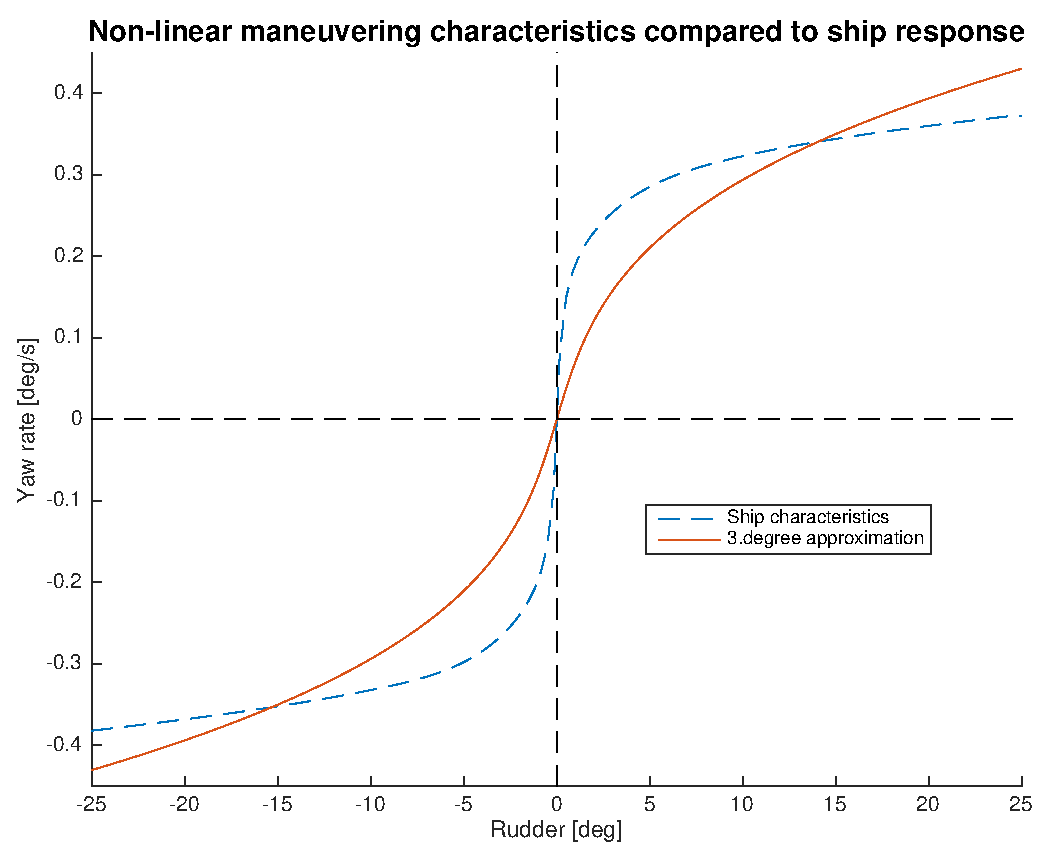
\includegraphics[width= \textwidth]{task1.4/Task1_4_Nomoto2_delta_r}
    \caption{Approximation of ship characteristics}
    \label{fig:nomoto2_delta_r}
\end{figure}

When curve fitting this model to the ship, the errors in the estimated ship characteristics becomes very clear. Since the steady-state is $b_3 r^3 + b_2 r^2 + b_1 r = \delta$, and we can see from figure \ref{fig:nomoto2_lin} that the only rudder angle where the actual and estimated curves intersect is at $\delta = 17\degree$, this is the only rudder angle where the steady-state model solution will match the ship as seen in figure \ref{fig:nomoto2_nonlin}.
    
\begin{figure}[H]
    \centering
    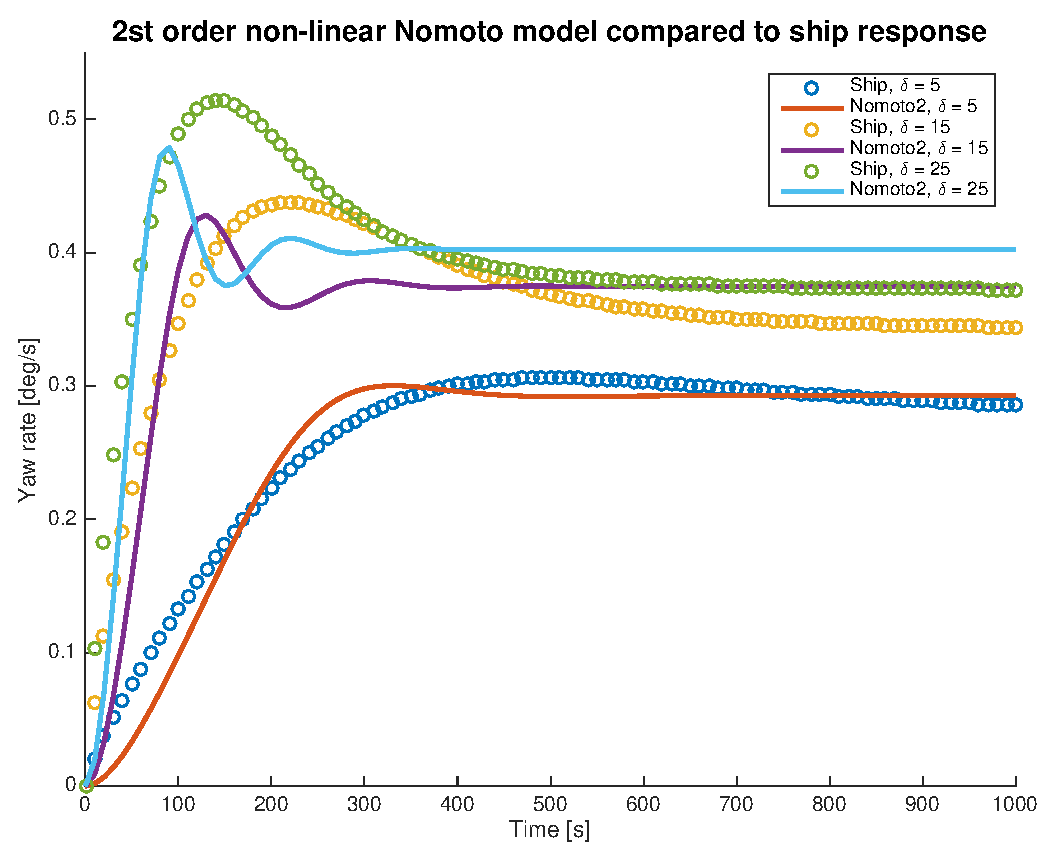
\includegraphics[width=  \textwidth]{task1.4/Task1_4_Nomoto2_curvefit}
    \caption{2.order non-linear Nomoto model}
    \label{fig:nomoto2_nonlin}
\end{figure}

\subsubsection*{1. order non-linear Nomoto}
Norbins' extension of the linear first order model:
\begin{equation}
\begin{split}
	T\dot{r}+H_N(r)=K\delta \\
	H_N(r) = n_3r^3 + n_2r^2 + n_1r + n_0
\end{split}
\end{equation}
Where the steady state of $H_N(r)=K\delta$. We know from Fossen(2011) that $n_i = \frac{b_i}{|b_1|}$, and since our ship is stable we know that $n_1=1$, and $n_3 = sign(b_3)=1$ thus resulting in following model.
\begin{equation}
\begin{split}
	T\dot{r}+r^3 + r=K\delta 
\end{split}
\end{equation}
When curve fitting this model we got as expected a response which is not able to follow the overshoot to the ship as seen in figure \ref{fig:nomoto1_nonlin}.

\begin{figure}[H]
    \centering
    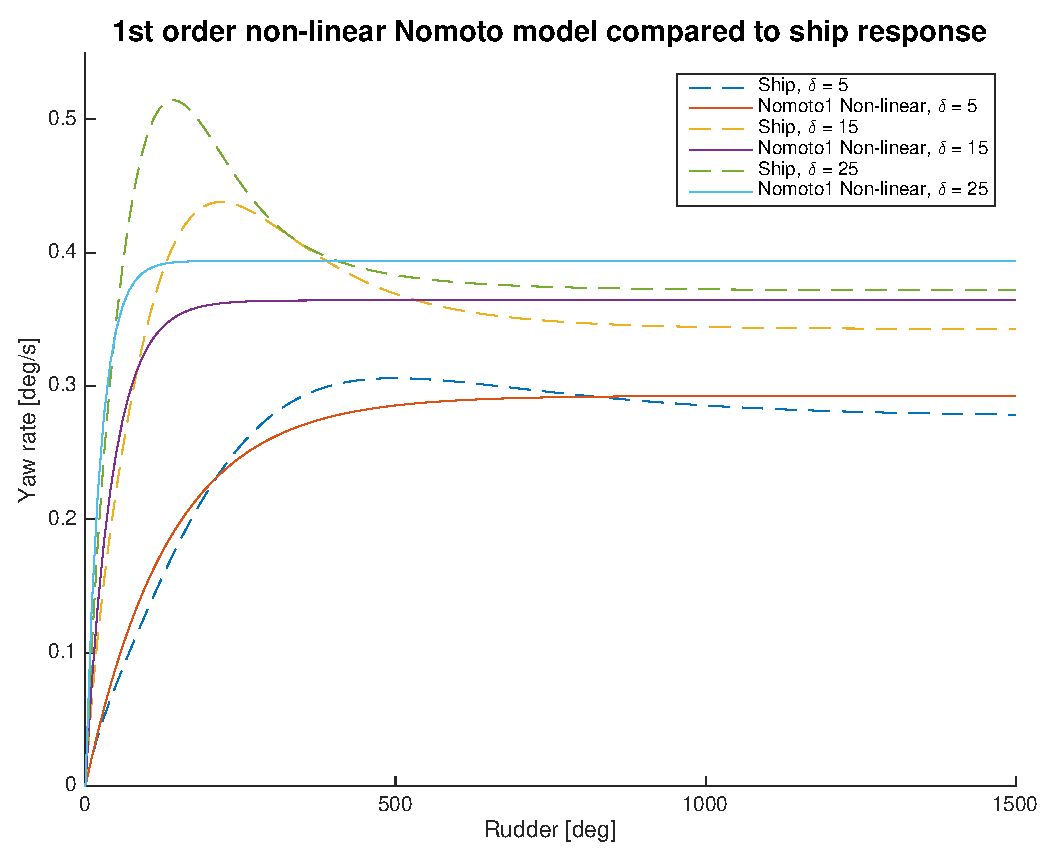
\includegraphics[width=\textwidth]{task1.4/Task1_4_Nomoto1_curvefit}
    \caption{1.order non-linear Nomoto model}
    \label{fig:nomoto1_nonlin}
\end{figure}

\subsubsection*{Heading model conclusion}
Both first order models where not able to follow the overshoot and oscillations to the ship, and would therefore make a poor model. The second order model with non-linearities was hard to get good steady-state solution on, and was very hard to do curve fitting on. Which in turns means that the model preformed bad. This leaves us with the second order linear model which where easy to curve-fit to the original response, and preformed quite well. This is the model we are using through the rest of the assignment, with an added integrator for heading. 
\begin{equation}
    \frac{\psi}{\delta}(s) =0.03 \frac{(1+320 s)}{s(1+130 s) (1+150 s) } \\
\end{equation}

\subsubsection*{Heading control law}
When using a linear model, the obvious choice of controller would be a PID. We have a stable ship under the influence of current, so we need at least a PI-controller. We ended up using this controller.